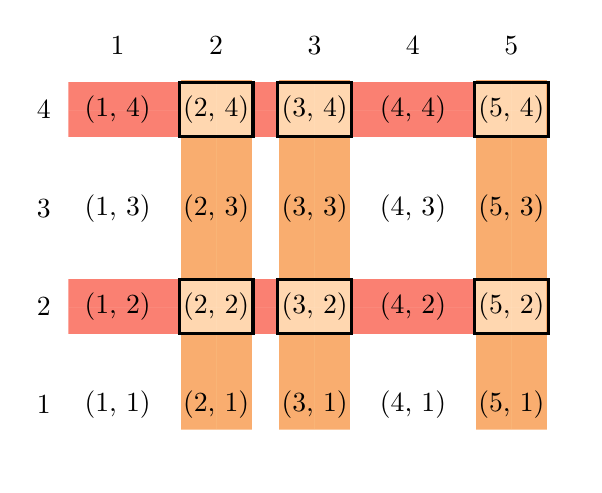
\begin{tikzpicture}
[
scale = 1.25,
v/.style = {Apricot, line width = 9mm},
h/.style = {Salmon, line width = 7mm},
rect/.style = {very thick}
]
\foreach \i in {1, 2, 3, 4, 5}{
	\foreach \j in {1, 2, 3, 4}{
		\coordinate (hs\j) at (.5, \j);
		\coordinate (he\j) at (5.35,\j);
		\coordinate (vs\i) at (\i, .75);
		\coordinate (ve\i) at (\i, 4.3);
	}
}
\begin{scope}[blend mode=screen]
\filldraw[v] (vs2) rectangle (ve2);
\filldraw[v] (vs3) rectangle (ve3);
\filldraw[v] (vs5) rectangle (ve5);
\filldraw[h] (hs2) rectangle (he2);
\filldraw[h] (hs4) rectangle (he4);
\end{scope}
\foreach \i in {1, 2, 3, 4, 5}{
	\foreach \j in {1, 2, 3, 4}{
		\coordinate (\i\j) at (\i, \j);
		\node (n\i\j) at (\i\j) {(\i, \j)};
		\coordinate (obl\i\j) at (\i -.375, \j -.275);
		\coordinate (otr\i\j) at (\i + .375, \j + .275);
	} 
}
\foreach \i in {1, 2, 3, 4, 5}{
\node at (\i, 4.65) {\i};
}
\foreach \i in {1, 2, 3, 4}{
\node at (.25, \i) {\i};
}
\draw[rect] (obl24) rectangle (otr24);
\draw[rect] (obl54) rectangle (otr54);
\draw[rect] (obl34) rectangle (otr34);
\draw[rect] (obl22) rectangle (otr22);
\draw[rect] (obl32) rectangle (otr32);
\draw[rect] (obl52) rectangle (otr52);
\end{tikzpicture}
